\chapter{Bilancia di Cavendish}
\section{Introduzione}
\subsection{Oggetto della ricerca}
Misurazione della costante di gravitazione G mediante la bilancia di Cavendish.
\subsection{Proprietà geometriche dei corpi e strumentazione}

\begin{tabular}{ll}
m=38.3$\pm$0.2 g & massa sfere piccole\\
M=1500$\pm$10 g	 & massa sfere grandi\\
r=9.53 mm & raggio sfere piccole\\
R=31.9 mm	 & raggio sfere grandi\\
$m_c\cong 2m$ & massa manubrio\\
\end{tabular}


\begin{center}
 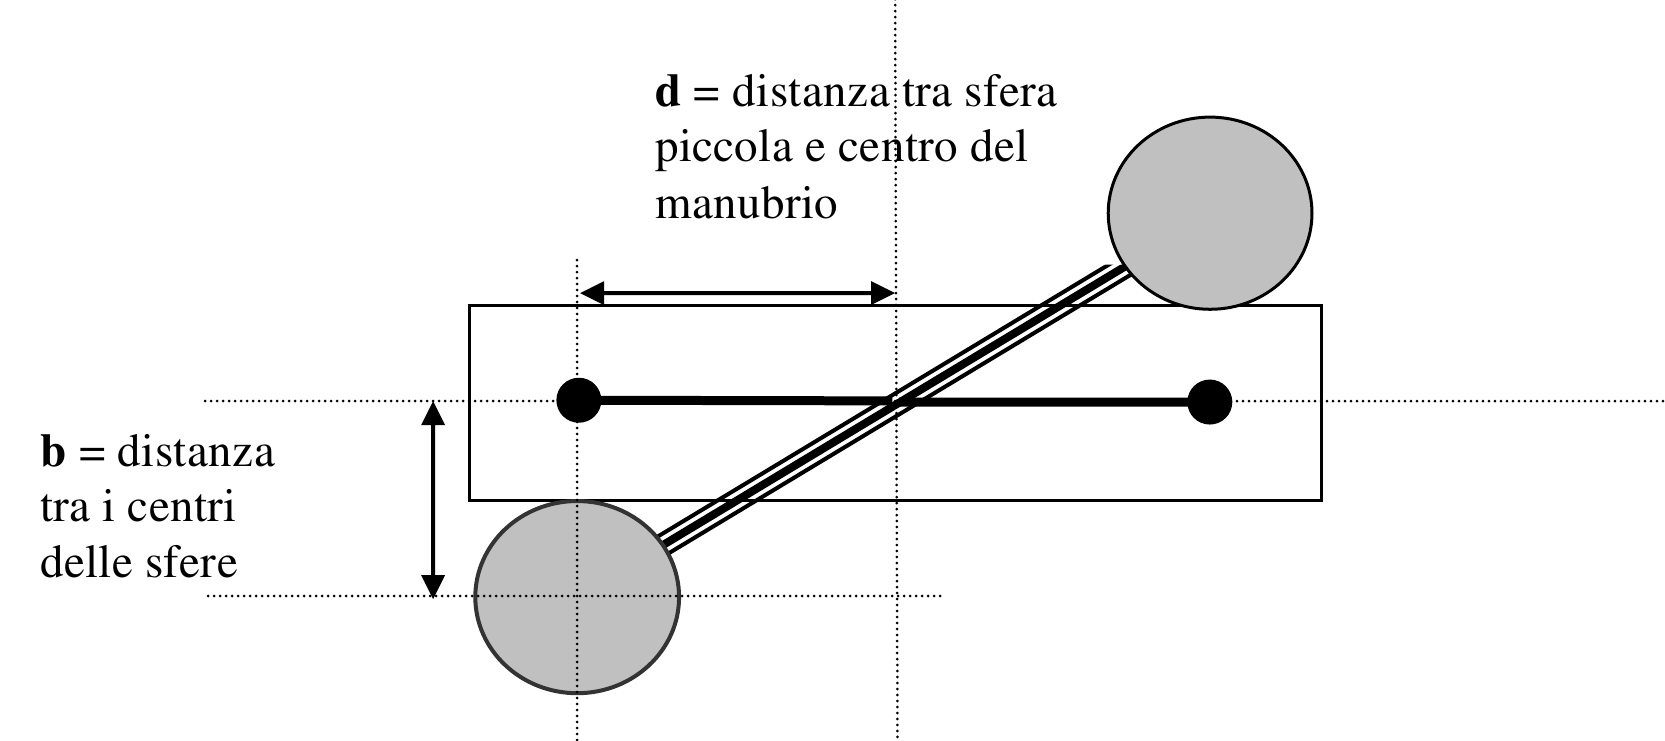
\includegraphics[scale=0.25]{../grafici/cavendish/schema.png}
\end{center}

Il momento d'inerzia $I$ del corpo si calcola:

$$ I=2m(d^2+2/5r^2)$$
L'inerzia del corpo è:
$I = 1.94283 \cdot 10^{-4} kg\cdot m^2$
L'incertezza sul momento di inerzia è dell'ordine di $10^{-6}$, ed è perciò trascurabile. 
\subsection{Metodo in breve}
La bilancia di Cavendish è uno strumento estemamente sensibile utilizzato per misurare forze di bassissima entità. Il principio su cui si basa è quello dell'equilibrio tra due momenti torcenti: quello della forza di gravità e quello dovuto alla torsione del filo. Questo equilibrio non si raggiunge istantaneamente, ma è necessario attendere un certo tempo, entro il quale il pendolo oscillerà (in modo smorzato).

Per trovare la posizione di equilibrio basterà ricercare una media (mobile) tra i le posizioni di massimo e di minimo.

\begin{center}
 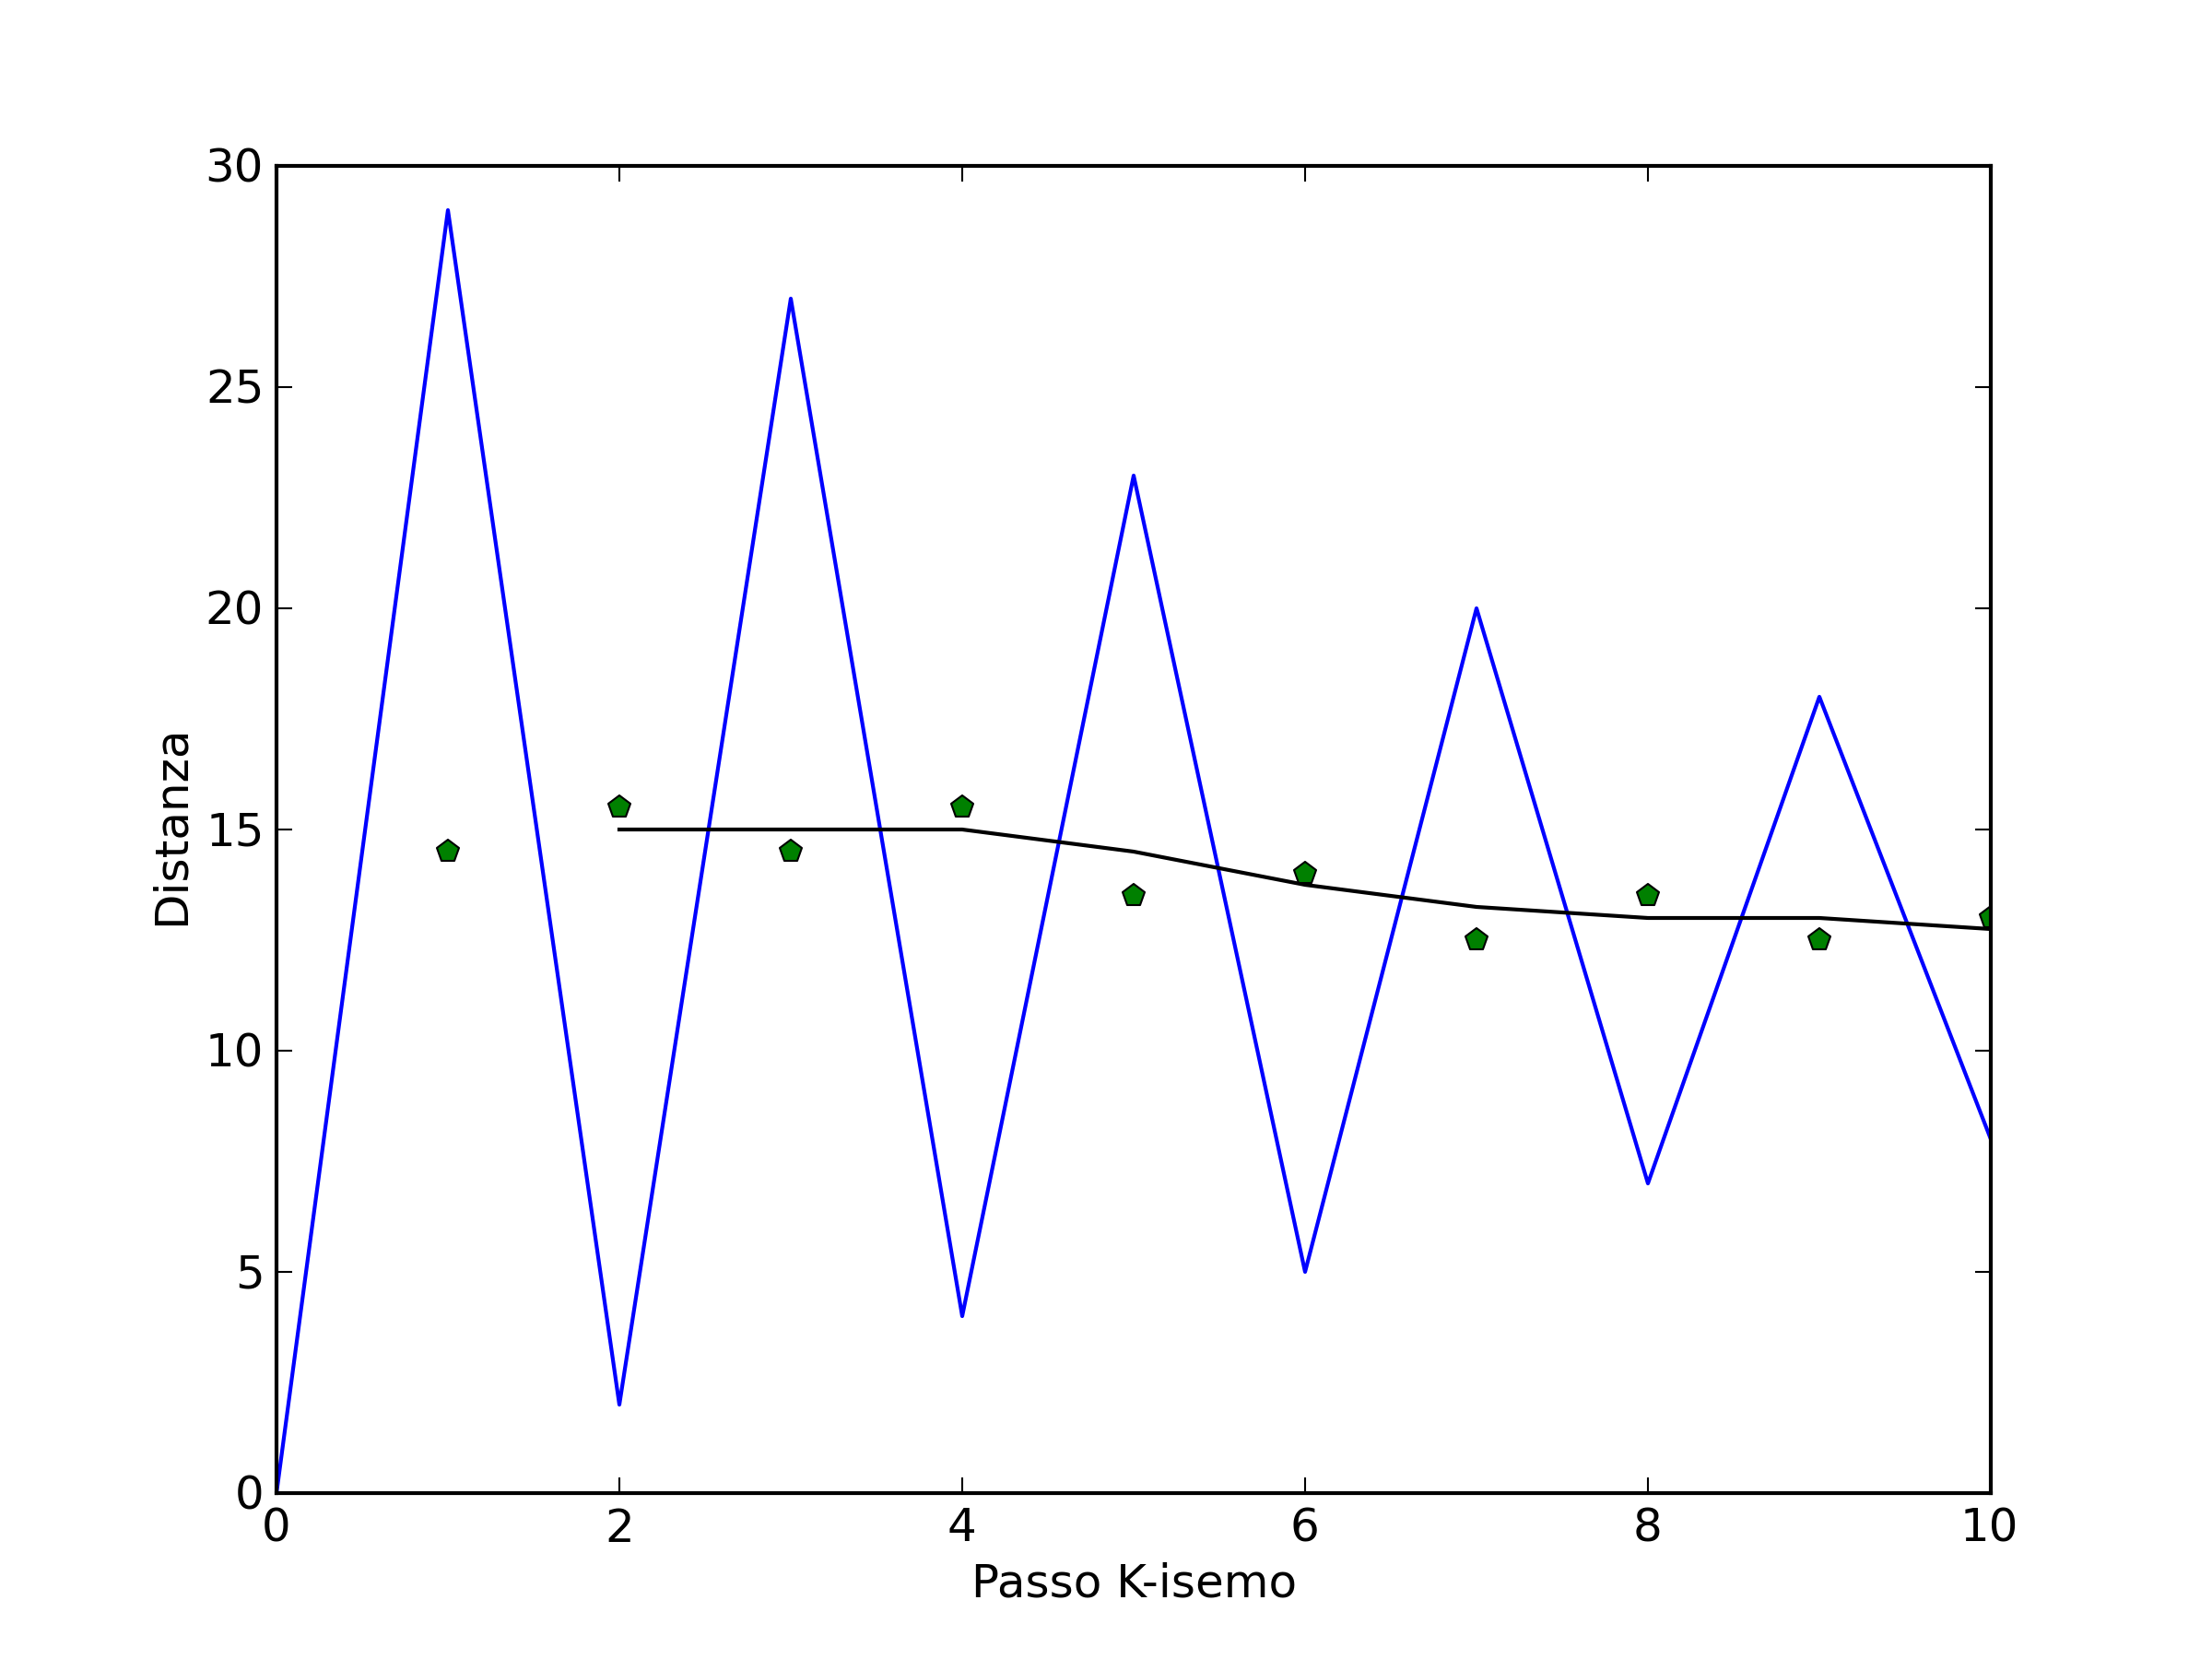
\includegraphics[scale=0.50]{../grafici/cavendish/oscillazioni.png}
\end{center}

Essendo le oscillazioni del pendolo molto piccole, queste vengono amplificate grazie a un laser, che viene fatto incidere sul pendolo, e viene riflesso su di una parete distante circa 5.50 m.

La posizione di equilibrio e le varie misurazioni sulla posizione del pendolo vengono effettuate su di un nastro di carta graduata attaccata alla parete.


\section[Misura di k e theta]{Misura $k$ e $\theta$}
L'incertezza relativa allo strumento per la misurazione del periodo è trascurabile rispetto l'entità della misura. 
Il periodo misurato è ottenuto come media di 5 periodi.

$$T = 508 \pm 20 \ s$$

Per ricavare $k$, ricordiamo che:
$$T^2 = 4 \pi^2 \frac{I}{k}$$
Quindi
$$k = 4 \pi^2 \frac{I}{T^2} = 2.84 \cdot 10^{-8}\ kg\cdot m^2/s^2$$


$$G = \frac{k \theta b^2}{2mMd} = 5.85 \cdot 10^{-11}\ qualcosa$$

\section{Analisi dati} 

periodo = 512.8
$ine = 1.94283*10^-4$
dist = 5.50
b = 0.0465
d = 0.05
mp = 0.0383
Mg = 1.500

Correzione:
Bisogna applicare una correzione di 1.07 a G, data dall'attrazione che c'è tra le altre due sfere, che tende a fare ruotare il pendolo in senso opposto.

$$ G_c = 1.07\cdot \frac{\theta k b^2}{2mMd} = 6.26\cdot 10^{-11}\ qualcosa$$

\section{Conclusioni}
